\chapter{なぜ今の文章はみな同じように聞こえるのか}

この講義には、文字どおりの黒板数学は含まれていない。黒板上の導出も、記号操作も、スライドから回収すべき公式もない。だが、議論にはなお数学的な背骨がある。Macfarlane は、一つの書き方がいかにして一つの経験のかたちに応答しうるのかを問い続け、司会者はその問いを、局所的で精密なものになるまで研ぎ澄ませていく。したがってこの講義は、区別、梯子、パイプライン、尺度、そして agency の変形を通して展開される。伝記から始まり、光へと転じ、散文の微細な mechanics に入り、process と world view へ広がり、そして最後に、revision、precision、そして平板化に抗して distinctiveness を守ることへと至る。

\begin{remark}
この章の公式は、講義が speech の中で明示している構造を図式的に述べたものである。講義中の記法を回収したものではない。話の形式的な論理を明らかにするところでのみ用いる。
\end{remark}

\section{山、光、そして捉え損なうこと}

講義は、正しい場所から始まる。教義からではなく、admiration と origin からである。司会者は、Macfarlane の感受性がどこから来るのかを問う。Macfarlane は、それに talent ではなく training の言葉で答える。彼は mountains の中で育った。mountains は感覚を sharpen し、alertness を要求し、自己のふだんの殻を削り落とす。したがって danger は、付随的な背景ではない。知覚の engine の一つなのである。

講義の最初の因果連鎖は、図式的には
\begin{equation}
\text{danger} \longrightarrow \text{alertness} \longrightarrow \text{openness} \longrightarrow \text{attention}.
\end{equation}
と書ける。これはすでに autobiography 以上のものである。書き手がいかに形成されるかの説明なのだ。より明るい光、より鋭い雪、鼻の中で wire のように感じられる空気、risk assessment、身体の露出。これらはすべて、気づきの様式となる。mountains は、単に scenery を供給するのではない。感覚の教育を供給するのである。

この冒頭から、司会者は最初の決定的な転回を行う。``その obsession with light について話してください。'' そして彼は、飛行機から夕焼けを photograph しようとして失敗したばかりの fresh な anecdote を語り、その場面が記憶の中で薄れていき、ついには十分に言葉にできないままになるかもしれないと悟った grief を口にする。この grief は重要である。これを飛ばしてしまうと、この講義を本当に動機づけている問題を失う。Macfarlane は abstract aesthetics から始めるのではない。ある特定の intense な seeing の前で、language が足りないと感じられる、その感覚的な inadequacy から始めるのである。

彼の答えは二段階で来る。まず彼は、speech の中でその sunset を intensify する。彼が言うように、そこにはほとんど slaughter に近いもの、血のようで wild なものがあった。ついで一歩引いて、形式的な lesson を述べる。subject が light であるとき、language はいつでも遅れているのだ。

講義の核心的な opposition はここに現れる。
\begin{align}
\text{correspondence} &\not\Rightarrow \text{light を適切に書くこと},\\
\text{artifice} &\Rightarrow \text{知覚の喚起}.
\end{align}
もし correspondence にしがみつくなら、language を対象に一点一点ぴたりと合わせようとする futile な quest の中に閉じ込められたままである。Macfarlane の recommendation は、もっと radical で、もっと liberating だ。その quest を abandon せよ、というのである。言葉が scene を point for point に reproduce しなければならないと insist するのをやめた瞬間、metaphor、distortion、formal construction が、それ本来の仕事をすることを許される。

\begin{definition}
この講義における \emph{representation of perception} とは、thing in itself ではなく、movement、mood、history、attention を通してある encounter の中に到来したものとしての thing を意味する。
\end{definition}

だからこそ、司会者の impressionist への analogy はこれほどよく当たる。Monet は、scene を paint の中に imprison しようとしているのではない。scene の impression を描いているのだ。Macfarlane も prose で同じ move をする。彼は ``capture'' という verb にさえ抵抗する。nature を capture するということ自体、すでにそれを captive として思い描くことだからである。よりよい verb は evoke だ。この distinction が据えられると、講義は light から、form と movement がさらにあからさまに不可分である別の medium、すなわち water へと進むことができる。

\section{水、句読点、そして思考の小さな mechanics}

water は新しい topic として現れるのではない。anti-correspondence method を最初に持続的に試すものとして現れる。Macfarlane は river の本を何年も書いてきた。そしてその長い labor から、ひとつの強い形式的結論を引き出す。水には単一の grammar など存在しない。この一点の上に、この節の残りすべてが回転している。

ここで司会者が有益なのは、彼がただちに abstraction を grounding するからである。rivers はすべて同じ仕方で動くのではない。still であり、pooled であり、meandering であり、straight であり、rapid でありうる。彼がそう言った瞬間、Macfarlane は lesson を sharpen できる。
\begin{equation}
\text{river language} \neq \text{ただ速いだけの language}.
\end{equation}
この修正は重要である。もし ``flow'' という metaphor が、すべての waters を一つの prose texture の中へ collapse してしまうなら、それは弱すぎる。flat な lake water、turning する river water、wild な rapid water は、それぞれ異なる rhythms、tones、sentence structures を要求する。

講義自身の progression に従えば、この river taxonomy は prose taxonomy になる。
\begin{itemize}
\item pooled または still な water は、遅れ、広がり、pause を求める
\item meandering な water は、drift、turn、穏やかな redirection を許す
\item straight な water は、propulsion と line を許す
\item rapid な water は、urgency、accumulation、impact を要求する
\end{itemize}

そこから話は、大きな form から小さな operators へと狭まっていく。Macfarlane は、自分を preposition obsessive であると同時に punctuation obsessive でもあると呼ぶ。dash が最初に来る。full stop は、彼によれば、硬い終わりを bang と打ち下ろす。dash は liquid のままである。その中を meaning は backward に eddy することも、forward に flow することもできる。これは ornament ではない。syntax が motion を seal off せずに manage する仕方の model なのだ。

その次に prepositions が来る。そしてここで講義は異様に exact になる。preposition は filler ではない。それは書き手と world との metaphysical relation 全体を変える。
\begin{equation}
\text{about river} \longrightarrow \text{with river} \longrightarrow \text{by river}.
\end{equation}
river について \emph{about} 書くことは、それを object として記述することである。river と \emph{with} 書くことは、すでにそれにある種の co-authorship、少なくとも thought における co-presence を与える。river によって \emph{by} 書かれることは、さらに先へ進む。書き手は conduit になり、channel になり、medium になる。司会者はすぐにこの force を認め、より plain に言い換える。まるで river が co-author にさえなるかのようだ、と。この言い換えは notes に残すべきである。なぜなら講義は繰り返し、まさにこの仕方で前進するからだ。Macfarlane が distinction の圧力を与え、司会者がそれを、より pedagogical な sentence へ圧縮するのである。

rhythm が次の narrowing である。poetry は私たちに rhythm を expect させる。だが Macfarlane によれば、nonfiction もまた、読者の ``mind's ear'' に作用する。それは proposition だけで働くのではない。sound、pattern、cadence、internal rhyme によって働くのだ。だからこそ彼は first lines に এত इतना? no, need Japanese: এত? Let's correct. We need avoid accidental noise. Continue properly.

それは proposition だけで働くのではない。sound、pattern、cadence、internal rhyme によって働くのだ。だからこそ彼は first lines にこれほど長くこだわる。first line は、いくつもの仕事を同時にしなければならず、講義は事実上、ひとつの簡単な model を与えてくれる。
\begin{equation}
\text{first line} = \text{sound pattern} + \text{puzzle} + \text{conceptual opening}.
\end{equation}

``The wind was rising, so I went to the wood'' は、この講義でもっとも幸福な instance である。それは alliteration と rhythm と puzzle を一度に与える。wind が rising しているのに、なぜ wood へ入っていくのか。これは単に pretty な phrasing ではない。小さな narrative engine なのである。これに対して、``12{,}000 years ago, a river is born'' は、講義が言うように、rhythmic さでは劣るが、より ominous である。それは露骨な sound を、temporal な vastness と conceptual な mystery と交換している。

Macfarlane はさらに、internal sound pattern の中へ細かく押し入っていく。``White as eyes'' と ``rises and flows'' は互いに echo し始め、argument が laid out される前から、text は読者に作用し始める。これが、この講義の重要な reminder である。nonfiction は nonfiction だからといって、flatly propositional である必要はない。

この時点で ground work は敷かれた。water は formal principle となり、punctuation と prepositions は real operators に昇格し、rhythm は nonfiction に返還された。ここでようやく司会者は、この講義で最も明快な局所的 craft question を問うことができる。

\section{書く速さを、形式上の問題として考える}

\subsection{Question \& Answer}

\paragraph{Question.} speed はどう書くのか。

\paragraph{Answer.} ``sentences を短くせよ'' のような crude な rule によってではない。この講義の答えはもっと精密である。syntax を tumble させ、contract させ、読者に容易な rest の場所を与えないように組み立てることによって、speed は書かれる。

Macfarlane は、司会者が問う権利を十分に earned した問いに対し、まさにそうする。彼は example を出す。それ以上に、講義は example 自体を screen に載せる。そこに pedagogy についての何かが示されている。彼は fast prose を abstract に記述しているだけではなく、specimen を一旦止めて inspect しているのである。

\begin{figure}[ht]
\centering

\includegraphics[width=0.92\textwidth]{lecture_17_figure_02.png}
\caption{speed と panic の syntax を例示する on-screen の river passage}
\end{figure}

この screenshot は、evidence として重要である。そこには visible な equations も lecture diagrams もない。prose block それ自体が exhibit なのだ。この quotation は dense で、accumulative で、ほとんど切れ目がない。theory が説明される前に、目はすでに pressure に出会っている。

Macfarlane の説明は、簡潔には
\begin{equation}
\#(\text{and}) \uparrow,\qquad \ell_{\text{clause}} \downarrow,\qquad a_{\text{verb}} \uparrow
\Longrightarrow \text{panic and speed} \uparrow.
\end{equation}
と書ける。ここで \(\ell_{\text{clause}}\) は average clause length、\(a_{\text{verb}}\) は increasingly active な verbs が及ぼす pressure を表す。

彼はまた、ひとつの crucial な局所的 equivalence を与える。
\begin{equation}
\text{``and''} \sim \text{dash}.
\end{equation}
つまり、この種の prose において conjunction は、先ほど dash がしていた仕事をする。それは line を走らせ続ける。calm な hierarchy を妨げる。full stops と neat な subordination によって組織された sentence の、stop-start の composure を拒むのである。

導出は単純だが、exact である。講義自身の order に従って、こう述べることができる。
\begin{enumerate}
\item きれいに bounded された clause から始めるのではなく、すでに moving している sentence の内部から始める。
\item ``and'' を反復し、一つの unit が次のものへこぼれ込み続けるようにする。
\item conjunction のあいだの clauses を、より短く、より速くする。
\item verbs の pressure を高める。slammed、exploded、punching、ramming、hauling。
\item ``river'' において article を落とす。そうすることで、その force は named object という感じをやめ、いたるところで一挙に acting する medium のように感じられ始める。
\item 結果として、読者は breathless になる。なぜなら syntax が、breath と hierarchy がふつう回復される points を withholding するからである。
\end{enumerate}

article を落とすというのは、とりわけ強い小さな move である。``The river'' は、私たちが距離を取って立てる thing である。``River'' は、more like agency、more like impact、less like scenery に感じられる。取るに足りない grammatical subtraction が、scene の ontology を変えるのだ。

screen は prose block を与えるだけで、analytic diagram は与えない。したがって、ここで私たちが加える any diagram は、はっきり secondary なものにとどまらなければならない。ゆえに次のものは、recovered lecture graphic ではなく、editorial reconstruction である。

\begin{figure}[ht]
\centering
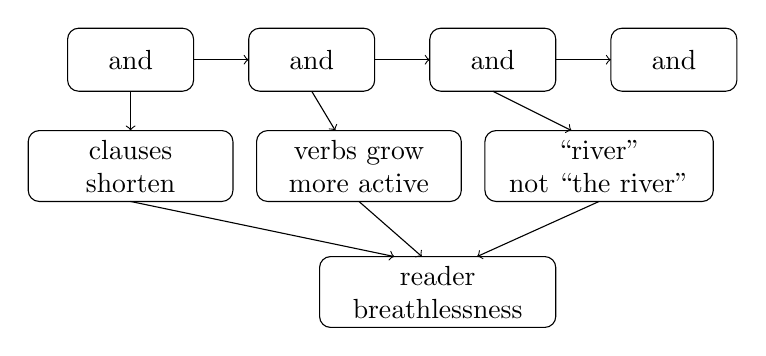
\begin{tikzpicture}[x=1cm,y=1cm]
\draw[rounded corners] (-5.2,1.2) rectangle (-3.6,2.0);
\node at (-4.4,1.6) {and};
\draw[rounded corners] (-2.9,1.2) rectangle (-1.3,2.0);
\node at (-2.1,1.6) {and};
\draw[rounded corners] (-0.6,1.2) rectangle (1.0,2.0);
\node at (0.2,1.6) {and};
\draw[rounded corners] (1.7,1.2) rectangle (3.3,2.0);
\node at (2.5,1.6) {and};

\draw[->] (-3.6,1.6) -- (-2.9,1.6);
\draw[->] (-1.3,1.6) -- (-0.6,1.6);
\draw[->] (1.0,1.6) -- (1.7,1.6);

\draw[rounded corners] (-5.7,-0.2) rectangle (-3.1,0.7);
\node[align=center] at (-4.4,0.25) {clauses\\shorten};

\draw[rounded corners] (-2.8,-0.2) rectangle (-0.2,0.7);
\node[align=center] at (-1.5,0.25) {verbs grow\\more active};

\draw[rounded corners] (0.1,-0.2) rectangle (3.0,0.7);
\node[align=center] at (1.55,0.25) {``river''\\not ``the river''};

\draw[rounded corners] (-2.0,-1.8) rectangle (1.0,-0.9);
\node[align=center] at (-0.5,-1.35) {reader\\breathlessness};

\draw[->] (-4.4,1.2) -- (-4.4,0.7);
\draw[->] (-2.1,1.2) -- (-1.8,0.7);
\draw[->] (0.2,1.2) -- (1.2,0.7);

\draw[->] (-4.4,-0.2) -- (-1.05,-0.9);
\draw[->] (-1.5,-0.2) -- (-0.7,-0.9);
\draw[->] (1.55,-0.2) -- (0.0,-0.9);
\end{tikzpicture}
\caption{on-screen の river passage の背後にある mechanics の editorial reconstruction}
\end{figure}

この効果全体に対する講義自身の phrase はすばらしく、そのまま残すべきである。これは ``syntax of panic'' なのだ。その achievement は、その sentence が panic を \emph{describe} することにない。panic の制御された analog を、読者に experience させることにある。

ここから司会者は、正しい次の一手を打つ。もし sentence をこのように build できるのなら、そのような sentences はどこから来るのか。

\section{notebook から本へ}

\subsection{Question \& Answer}

\paragraph{Question.} notes は、どうやって books になるのか。

\paragraph{Answer.} notebook の中にすでに隠れていた tiny な完成済みの本を、ただ expansion することによってではない。講義は insist する。notes は、最初は fragmentary であり、encrypted であり、しばしば noncommunicable でさえある。本とは、notes がすでにそうであるものではない。それは、return、recovery、pattern recognition のもとで、notes がなっていくものなのだ。

ここで講義の rhythm は変わる。river sentence の urgency のあとで、Macfarlane は意図的に speed を落とし、いわば、段階に分けてみよう、と言う。この pacing は重要である。司会者は sentence mechanics から book mechanics へと shift しており、Macfarlane は epigram ではなく process を与えることによって答えている。

第一段階は fieldwork である。これらの books は何年もかかり、多くの journeys と、人々や rivers や mountains との反復的な encounters を要する。Macfarlane は A6 ほどの small notebooks を好む。実際の conditions のもとで carried され、bent され、used されうるからだ。そこへ彼は、半ば冗談めかして \emph{qualia} と呼ぶものを書き込む。bits、bobs、対話の fragments、image の flashes、mind に stick する pebbles や feathers である。

これらの notes は orderly ではない。discontinuous である。これが、この講義のもっとも強い実践的 points のひとつだ。encounter の瞬間には、finished prose のための time はない。書き留めて、次へ moving on するしかない。その日の終わりに jotting することも重要になる。headlamp をつけ、memory が cool down する前に、brain から fresh に notes を pull out するのだ。

司会者はそのあと、すばらしい metaphor を寄与する。page は condensation surface になる。thought は vapor のようにそこにあった。paper が、それを gather させるのだ。Macfarlane はこの point を引き取り、さらに強める。paper と pen は、keyboard と pixel がしない何かをする。notes は ``fresh from the fire'' であり、まだ hot く、まだ別の reader のために shaped されていない。

この notebook-to-book pipeline は、
\begin{equation}
\text{fragment} \longrightarrow \text{mnemonic trigger} \longrightarrow \text{memory expansion} \longrightarrow \text{pattern recognition} \longrightarrow \text{heart work}.
\end{equation}
と書ける。

この chain の middle part は、とくに強調されるべきである。Macfarlane が home に戻り、screen 上で notebooks を読み返すとき、それぞれの fragment は一本の糸の visible な端になる。その糸を pull すれば、周囲の scene 全体がふたたび開いてくる。これが、この講義における recall のもっとも exact な phenomenology である。note は experience そのものではない。それは、experience に再入場するための handle なのである。

この地点で Macfarlane は Rilke を持ち出すが、慎重に、そして paraphrase のかたちでそうする。このあたりの transcript は unstable だが、distinction 自体は secure である。
\begin{equation}
\text{notebook work} \longrightarrow \text{heart work}.
\end{equation}
immediate notation は、finished labor ではない。hard work は、images が再訪され、相互に relate され、その resonance の中で理解され始めるときに始まる。

だからこそ講義は、そのあと open hand へと向かう。この example がすぐれているのは、あとから恣意的に選ばれたのではないからだ。Macfarlane はその hand に、まず cave stencil art の中で気づく。hand の mark ではなく、その absence の mark としてである。その image は、後の別の journeys や別の media の中で再帰する。それは social form の中でさえ再帰する。greeting や welcome として。孤立した image として始まったものが、motif になるのだ。

この emergence は、より精密には
\begin{equation}
\text{反復される image} \longrightarrow \text{journeys をまたぐ recurrence} \longrightarrow \text{pattern が lighting up する}.
\end{equation}
と表現できる。``lighting up'' という phrase が鍵である。motif は、単に repeated されるのではない。active になるのだ。書き手がそれを見る。読者もまた、それを見ることができるようにされる。

ここで司会者は有益にこの point を言い直す。では、あなたが本当に記述しているのは pattern recognition なのですね。まさにそのとおりである。そして、この recognition こそが、encrypted な notes の pile を、形を持った本の beginnings へ変えるのである。

そのあと講義は、もっとも unromantic な advice を加える。そしてそれは pattern の話から直接 emerge しているがゆえに、ここに属する。ass on chair. 現れよ。第一の rule は work であり、第二の rule は patterns を探すことである。この二つは一緒に属している。

\section{wonder、scale、そして unlearning}

\subsection{Question \& Answer}

\paragraph{Question.} unlearn するとはどういうことか。

\paragraph{Answer.} この講義がこの問いに reach するのは、sentence craft と long-form process をすでに確立したあとである。この order は重要だ。unlearning は mystical な ornament として提供されるのではない。attention し、patterning し、naive correspondence を distrust することをすでに学んだ writer の、より大きな epistemic consequence として提供されるのである。

直近の opening は、Macfarlane の息子についての anecdote である。彼は \emph{Is a River Alive?} という本を書いているのだと言う。すると子どもは、いわば、``Of course.'' と答える。司会者はすぐにこの force を見て取る。adults はしばしば、world との clear でありながら enchanted な relation を失ってしまう。children は、better argument を持っているのではなく、narrowed されていない ontology を持っているのかもしれない。

Macfarlane の最初の答えは wonder である。wonder は、彼によれば、本質的な survival skill である。rainbow が、この講義の specimen になる。この point は二つの方向へ同時に向けられる。第一に、wonder は freely given world の前で口があく astonishment である。第二に、wonder は explanation によって cancel されない。rainbow は、水によって constituent wavelengths へ分離された light として describe できる。だが、その explanation は experience を dissolve しない。むしろ science は、real を wonder から strip するのではなく、wonder へ finesse しうるのだ、と講義は示唆する。

そこへ Blake が入り、Blake とともに scale が入ってくる。一粒の sand は world へ開くことがある。tiny な poem は eternity の intimation を含むことができる。そこから Macfarlane は一般化する。
\begin{equation}
\text{micro scale} < \text{human scale} < \text{macro scale}.
\end{equation}
これはあくまで schematic notation にすぎない。講義の real point は strict ordering にあるのではなく、juxtaposition と nesting にある。私たちは ordinary には human scale に住んでいる。だが writer は、その scale を microscopic な order や cosmic な order の隣に置き、それらの tension を visible なままにしておける。

だからこそ講義は、microscope と telescope による early modern の scale の cracking-open を invoke する。Galileo は moon の上の mountains を見、van Leeuwenhoek は droplet の中の life を見る。Macfarlane にとって writing は、scales を collapse することなく互いに並置することで、これに似た act を perform しうる。

そこでようやく、司会者は ``blinders of rationality'' という phrase を導入する。これはまさに正しい transition である。Macfarlane はすぐに agree する。rationalist な habits の中で training された者にとって、river がその中の organisms の総和以上の意味で alive なのだと believe するには、unlearning が必要なのだ。彼はそのあと、この講義でもっともよい images の一つを与える。rationalism は、cave 全体を照らす floodlight ではなく、darkness の中を moving する一つの patch of light にすぎない。illuminated なその patch が私たちに think させるよりも、私たちはいつでも少ししか知らない。

river journey は、この philosophical turn の physical ground を提供する。ここで講義は一時的に numerical になる。
\begin{align}
Q_{\text{normal}} &\approx 150\,\mathrm{m^3\,s^{-1}},\\
Q_{\text{observed}} &\approx 275\,\mathrm{m^3\,s^{-1}},\\
\frac{Q_{\text{observed}}}{Q_{\text{normal}}} &\approx 1.83.
\end{align}
つまり river は、ordinary の rate のほぼ二倍で running していた。arithmetic 自体は simple だが、講義はそれをうまく使う。それは metaphysical claim を physical ordeal に anchor する。これは symbolic water のそばでの tranquil contemplation ではなかった。持続する tumbling、swimming、battering、exhaustion、日ごとの abrasion だったのである。

Macfarlane の formulation は忘れがたい。river が彼を unlearn したのだ。それは physical にそうしただけではなく、metaphysical にもそうした。それは、これは ``just water'' であり、ただの dead matter なのだ、という assumption を打ち破った。それは、自らを agency、presence、force、will として示し始めたのである。そしてそれは、journey の終わりにおける river-being、さらには godlike な presence の account へと culminate する。ここで講義は慎重である。language はその event 全体を carry しない。せいぜい、起こったことの analog を register できるだけだ。

それによって、私たちは earlier method へ戻ってくる。ここでも、いやおそらくはここでこそ、aim は perfect representation ではない。pressure の下での perception を exact に registration することなのである。

\section{questions は portal であり、他者は co-writers である}

\subsection{Question \& Answer}

\paragraph{Question.} 単純な question は、どうして whole book へ開きうるのか。

\paragraph{Answer.} 正しい question は、answer を待っている slogan ではないからである。それは、phrasing が最初に示唆するよりはるかに大きな chamber への narrow な opening なのである。

司会者はいま、Macfarlane の books に関するひとつの structural な特徴に名を与える。それらはしばしば、見かけは narrow な questions で始まる。Why climb mountains? Can a forest think? Does a mountain remember? Is a river alive? Macfarlane は agree する。だが structure を説明する前に、彼はひとつの failed answer に立ち止まる。George Mallory の ``Because it's there.'' である。有名ではある。だが useful では、実はない。本が inquiry を open のままにしておく必要がある、まさにその場所で、それを閉じてしまうからである。

講義の portal model は、次のように続く。
\begin{equation}
\text{simple question} \longrightarrow \text{narrow portal} \longrightarrow \text{複雑さの大きな chamber}.
\end{equation}
caving の example は、ここにふさわしい physical intuition を与えてくれる。人は small entrance を squeeze して通り、あるいは sump を dive してくぐり抜け、それからようやく vast な interior chamber に到達する。司会者の Narnia の analogy は、別の register で同じ point を sharpen する。wardrobe は modest だが、その向こうの world はそうではない。

これは、あとからつけられた mere metaphor ではない。Macfarlane は、それが自分にとって、こうした book-questions が実際には何であるかを crystallize する助けになると言う。それらは entrances なのだ。threshold においては modest だが、その先では expansive なのである。

そのあと講義は、ふたたび practical になる。portal question を見つけたなら、Macfarlane は未来の self に手紙を書く。books には何年もかかるので、book が forming しているあいだに、self も world も変わってしまう。だからその letter は commandment ではない。本が何になりうるか、どの metaphors が recur するか、それが world でどんな work をしうるかについての、provisional な declaration of hope なのである。

もう一つの aid もある。pinned quotations である。\emph{Is a River Alive?} のために、講義は Ursula Le Guin に戻り、とりわけ ``a great reach outward of mind and imagination'' という phrase に戻る。その quotation は、working injunction になる。question が door を unlock し、outward reach が、その中を歩いて入る能力を与えるのである。

そのあと司会者は、book-writing のどれくらいが plan で、どれくらいが adventure なのかを問う。Macfarlane は、もう一つの river analogy で答える。そしてこれは flatten してはならないほどよい。book は downstream へ rafting していく感じではなかった。それは river の中を upstream へ walking する感じだった。両足が planted されているときには stable である。progress が始まるのは、片足を lift した瞬間である。なぜならそのとき current が自分を off balance へ throw できるからだ。この lesson は、practical であると同時に conceptual でもある。book は、ただ存在するだけでは私たちを destabilize しない。次の一歩を踏み出させることによって、私たちを destabilize するのだ。

この答えは、自然に other people へつながる。Macfarlane は、people-less な old nature writing の version に抵抗する。companions、specialists、local knowers、astonishing voices で book を満たしたいのだ。司会者はすぐにその point を見て、それではそうした人々は almost co-writers なのではないかと問う。Macfarlane は spirit において yes と答え、講義の examples はその claim を正当化している。適切な person は、solitary な writer には決して supply できない forms of perception を本へ bring するのである。

conversation についての司会者の metaphor が、ここで central になる。一緒に fire を build することだ。これは正しい image である。conversation は単に content を exchange するのではない。どちらの speaker も alone では作れなかった heat と light を generate するのだ。Macfarlane はよろこんでこの model を writing の中へ import する。

講義はさらに、forms をまたいで widen する。poetry、libretti、songwriting、choral writing は、long-form prose writer に、prose だけでは隠れてしまうものを教える。singability、sound currents、一つの word から次の word への resistance、images が互いに live together することを許される loosness、そして slight mismatch の formal usefulness である。songwriting は彼を glitch の idea へ導く。それは error ではなく、productive friction である。off-beat な setting、uncanny な slippage、unresolved な contact は、strangeness を smooth away するのではなく、それを register したいときの formal resources になりうる。

これが、この講義の最後の late movement を準備する。book が portal question、future-self への letter、collaborators、そして wider な formal repertoire を持ったあとで、craft problem はもっと direct になる。precision、revision、bodily force、individuality を preserve しつつ、average prose へ押し戻されないでいるには、どうすればよいのか。

\section{precision、revision、そして distinctiveness}

司会者はこの turn を、まさにそうあるべき仕方で宣言する。``We've got to talk about words.'' 講義はいま fast な late run に入る。だがそれは miscellaneous ではない。title question に対する、集中的で practical な answer なのである。

Macfarlane は glossaries と place-words から始める。彼が unusual な words を使うのは、unusual に sounding するためではない。exact だからである。precision は、彼が insist するように、lyricism の enemy ではない。それは lyricism の instruments の一つなのだ。単一の local word が、perception の whole paragraph を compress することがある。``bone-cage'' や ``whale-road'' のような Old English の kennings は、language が metaphor と naming を fuse する能力を示している。Seamus Heaney の ``the palp and heft of language'' という phrase は、同じ tactile intelligence を指し示す。words は、扱われ、量られ、口と手の中で felt されうるのである。

講義はそのあと、Gaelic の place-names と place-words へ向かう。このあたりの transcript の spellings には、明らかに unstable なところがあるので、正確な orthography はのちに確認されるべきである。しかし、underlying point は secure である。多くの place-names は、shape、orientation、landscape relation を encode している。それらは、すでに存在している terrain に貼りつけられた mere labels ではない。attention の repositories なのだ。講義は、これを冗談めかして ``Gaelic positioning system'' と呼ぶ。だがその joke は、本物の formal insight を carrying している。language は topography を store しうるのだ。

ついで language death が現れ、講義はそれを unusually 明瞭に定義する。language は、その最後の living speaker が死に、その language がもはや passed on されなくなったときに死ぬ。records は残るかもしれない。transmission は残らない。そしてただちに、より強い claim が続く。
\begin{equation}
\text{language death} \longrightarrow \text{知識の喪失}.
\end{equation}
language は knowledge-storage system なので、ある種の knowledge はそれとともに vanish する。とりわけ、その knowledge が別の language へ clean に translate できないときにはそうである。したがって language death は、cultural であると同時に ecological な loss でもある。

講義はそのあと English 自体について問う。Macfarlane の答えは subtle である。あるとき English は glass のように transparent であるべきで、読者は medium を forget するべきである。別のときには、それは thick で rich で palpable であるべきで、読者は every word を feel するべきである。どちらの mode も misjudged されれば、prose は interference になる。choice が right なら、読者の body は language の weight や lift に participate する。この thought は、Heaney の ``palp and heft'' を一般的な craft principle へ延長する。すべての sentence が自らを announce すべきではない。すべての sentence が disappear すべきでもない。

revision が次に入り、ここで Macfarlane は、この講義でもっとも強い practical models を二つ与える。第一は potter model である。
\begin{align}
\text{wet mass of clay} &\longrightarrow \text{spin} \longrightarrow \text{shape} \longrightarrow \text{ornament},\\
\text{raw draft} &\longrightarrow \text{repeated passes} \longrightarrow \text{form} \longrightarrow \text{finish}.
\end{align}
point は decorative analogy にない。finished prose が clean に到来するという fantasy を拒むところにある。最初の material は muddy だ。form は、繰り返しの shaping を通じて emerge するのである。

第二の model は mosaic assembly である。
\begin{equation}
\text{set piece}_1 + \text{set piece}_2 + \cdots + \text{set piece}_n
\longrightarrow \text{assembly による chapter}.
\end{equation}
Macfarlane は linear drafting を requirement としない。ひとつの stretch が block するなら、別の stretch を先に書けばよい。本は pieces から built され、それから flow へと arranged される。これに paired されるのが、きわめて practical な二つの advice である。一日の work を終えるときには、次の sentence を known なまま残すこと。本当に stuck したなら、downstream へ jump して別の section を書くこと。どちらも、blockage を worship する代わりに motion を maintain する方法なのである。

講義の recurring refrain が、ここで力を伴って戻ってくる。ass on chair. 現れよ。たとえその日の成果が一 paragraph にすぎなくとも、book は一 paragraph 分 longer になっている。これは、この講義の中でもっとも glamorous でない line かもしれない。だが同時に、もっとも useful な line の一つでもある。

ついで automation が到来する。Macfarlane は、そのような tools が average prose に対してすることと、distinctive prose に対してすることとを区別する。grammar checkers は、多くの ordinary な sentences を改善する。だが同時に、deliberate な deviations を faults として flag する。彼自身の examples --- verbless paragraphs、fragments、abrupt paragraphing、syntactic strain --- は、まさに自動的 smoothing が dislike する प्रकार? Need Japanese. Continue correctly. Replace.

彼自身の examples --- verbless paragraphs、fragments、abrupt paragraphing、syntactic strain --- は、まさに automated smoothing が嫌う種類の writing なのである。formal tradeoff は、こう述べるのが容易である。
\begin{align}
\text{tool smoothing} \uparrow &\Longrightarrow \text{average competence} \uparrow,\\
\text{tool smoothing} \uparrow &\Longrightarrow \text{distinctiveness} \downarrow.
\end{align}
これは、この講義の終盤でもっとも clean な claims の一つである。writing が同じように聞こえるようになるのは、average acceptability に向けて repair されるときなのだ。

そのあと司会者は、別だが related な question を開き直す。language を visceral にするにはどうすればよいのか。答えは、先の ``capture'' の拒絶を extend するものであって、contradict するものではない。visceral writing は、event それ自体を capture しない。event の bodily analog を、読者へ transfer するのである。\emph{Underland} の claustrophobic な passages について語るとき、Macfarlane は William Golding の ``sympathetic kinesthesia'' という phrase を invoke する。読者の body は tighten し、speed up し、recoil する。これは anti-formal ではない。proposition の下で operating する formal power なのである。

こうしたことのあとでようやく、司会者は needless words を remove するという famous な rule へ戻る。Macfarlane の答えは partisan ではなく disciplined である。Walter Pater の ``hard, gem-like flame'' は、ひとつの valid な tradition を名づけている。Hemingway と Carver も、同様の subtractive line に立つ。だが Macfarlane は subtraction を universalize することを拒む。ある landscapes は removal を求め、別の landscapes は addition を求める。operative word は bespoke である。それぞれの encounter は、それ自身の density、それ自身の openness、それ自身の rhythm を求めるのだ。

この judgment は、astonishment についての講義の最後の remarks において、さらに重要になる。hyperbole は敵である、と彼は言う。purple prose は lie をつく。astonishment は、language を膨らませて shout させることによって best に render されるのではない。むしろ、それは precision、restraint、そして over-explain することの refusal によって better に serve される。ここで司会者は強い paraphrase を寄与する。every \emph{i} に dot を打ち、every \emph{t} に cross を打ってしまえば、私たちは reader に contemplate の余地も、sentence の上で stir する空間も残さないのだ。

それが、この講義を最後の elegant な portal idea への return へ導く。\emph{Is a River Alive?} の一文は、もし English に ``to river'' という verb がないのなら、river 以上に verb らしいものがあるだろうか、と問う。この line は complete であると同時に incomplete でもある。finished に感じられる。だが同時に、私たちを先へ送る。まさにこれこそが、この講義が good sentence に求める behavior である。局所的には shape を与え、全体的には mystery を残すこと。局所的には satisfy し、全体的には reopen すること。

\section{まとめ}

講義は mountains で始まり、distinctiveness で終わる。だがその progression は緊密である。dangerous な landscapes は alertness を train する。light を ``capture'' することの failure は、correspondence から artifice への shift を強いる。water は、prose がひとつの motion ではなく、多くの motions に応答しなければならないことを教える。punctuation と prepositions は real operators になる。speed は、serial coordination、contracting clauses、active verbs、そして ``river'' から article を落とすことによって書かれる。notes が books になるのは、return、memory-thread、pattern、heart work を通してのみである。wonder は writing の scale model へと widen し、さらに unlearning というもっと hard な demand へと widen する。books は、portal questions、future-self への letters、collaborators、そして expanded な formal resources によって organize される。writing の late craft は、precision、revision、bodily force、individuality を、smoothing と sameness に抗して defending することになる。

この講義の最後の claim は、最後の schematic relation 一つへと圧縮できる。
\begin{equation}
\text{attention} + \text{form} + \text{judgment} \Longrightarrow \text{distinctive prose}.
\end{equation}
これが title に対する practical な answer である。writing が同じように聞こえ始めるのは、それがその ear を、その pressure を、そして lived perception との exact な relation を失うときである。それがふたたび alive になるのは、syntax、rhythm、structure が、それらを呼び出した encounter に対して answerable にされるときなのである。